
	\section{Instruction set architecture: Branches, Function and stack}
	The main goal that ISA does is to put a \textbf{Contract} between the hardware and the software: If you are an hardware person, all you care about is the make your processor the fastest on the ISA. If you are a software person, you don't need to worry about the hardware behind anything, you only care about the software that you are building. This ISA gives a level of abstraction which makes it easier to develop better software/hardware.
	\begin{center}
	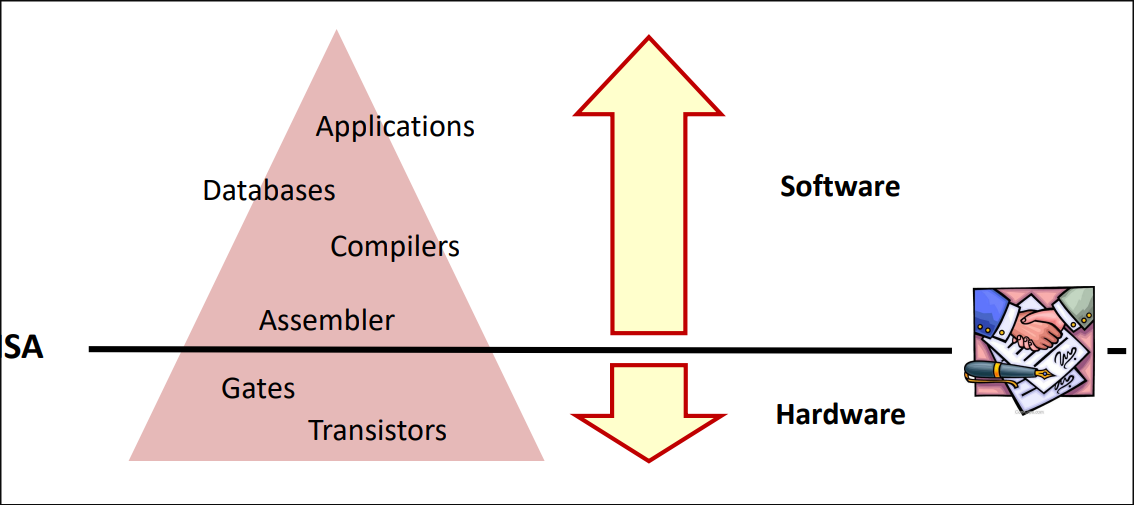
\includegraphics[scale=0.3]{screenshots/2025-10-11_6.png}
	\end{center}
	As we have seen in cs-173, arithmetic and logic operation are quite easy to understand and use in RISC-V. But here are some facts to know about them:
	\begin{itemize}
		\item Immediate constant takes at maximum 12 bits. The reason behind this is that the immediate part of the instruction is directly stored in the instruction, this means that there are 12 bits of the instruction that are reserved for the immediate part. Imagine having for instance a 30 bits immediate, then you would only have 2 bits for: the opcode, result register, input register ... 
		\item A way to go around this is to use the \texttt{.equ, num} and then to use \texttt{lui} directly on \texttt{num}. (this is possible because the assembler will directly translate the one line instruction into a three lines instruction). 
		\item Register \texttt{x0}, this register is \textbf{always} zero (by definition), you can write anything to this resgister, the value in it will always be zero. This can be useful  in a lot of case, it happens quite often that we need a zero in a instruction and the only way to do so would have been to \texttt{li} a register to 0 and then calling the instruction. Therefore, the \texttt{x0} register allows us to save instructions
	\end{itemize}

	\subsubsection{An if-then-else}
	To be able to do an if and else cause will need some branches, for instance if we wanted to translate the code:
	\begin{lstlisting}[language=c]
	if (x5 == 72) {
	   x6 = x6 + 1
	} else {
	   x6 = x6 - 1
	}
	...
	\end{lstlisting}
	Into RISC-V: it would look like this:
	\begin{lstlisting}[language={[RISC-V]Assembler}]
	.text 
		li x7, 72
		beq x5, x7, then_clause
	else_clause:
		addi x6, x6, -1 
		j end_if
	then_clause:
		addi x6, x6, 1 
	end_if:
		...
	\end{lstlisting}
	As you can see jump and branch are really similar however, there is a universal distinction between them:
	\begin{itemize}
		\item Jumps $\to $ \important{unconditional} control transfer instructions
		\item Branch $\to $ \important{conditional} control transfer instructions
	\end{itemize}
	However this is not the case for every assembly languages, for instance in x86, everything is defined as a jump.
	\subsubsection{A Do-while loop}
	\begin{center}
		A do while loop in c
	\end{center}

	\begin{lstlisting}[language=c]
	do {
	   x5 = x5 >> 1 
	   x6 = x6 + 1 
	} while (x5 != 0);
	...
	\end{lstlisting}

	\begin{center}
		A do while loop in risc-v
	\end{center}
	\begin{lstlisting}[language={[RISC-V]Assembler}]
	.text
	loop:
		srli x5, x5, 1 
		addi x6, x6, 1 
		bnez x5, loop 
	...
	\end{lstlisting}
	\subsection{Functios}
	In our high-level code, we usually use function to organized our code (Scala...) (those function can also be called methods, procedure dependeing of the context).\\ 
	What we would like is also to have function in assembly so that we don't have to write the same code always. What a function would look like is:
	\begin{enumerate}
		\item Place arguments where the called function can access them 
		\item jump to the function 
		\item Acquire storage resources the function needs 
		\item Perform the desired task of the function 
		\item Communicate the result value back to the calling program 
		\item realease any local storage resources 
		\item Return control to the calling program
	\end{enumerate}
	That sound pretty hard to do so let's do it step by step. First, the second and seven steps (I know).\\
	What we need is to jump to the function and the return. This is fairly easy to do, all we need is to call the jump instruction. For instance, let's call the function two times. This  would looks like this
	\begin{lstlisting}[language={[RISC-V]Assembler}]
	sqrt:
		...
		j back
	\end{lstlisting}
	And the main would look like this:
	\begin{lstlisting}[language={[RISC-V]Assembler}]
	main: 
		...
		j sqrt 
	back:
		...
		j sqrt 
	back2:
		...
	\end{lstlisting}
	However, isn't there an issue? what would happen if we tried to run this code?\\
	The answer is that this would lead to an infinite loop. the \texttt{sqrt} function doesn't know about the fact that there are more than one back.
	The solution to this problem is to:\\
	when you called the function, you store the current PC $+ 4$  (to go to  the next line) to a register (for instance \texttt{x1}). You then, call the function, do the computation there \textbf{and then} you rejump to the address store in the register \texttt{x1}.

	\begin{parag}{Jump and link}
		


	There is instruction that allows us to do this, those instruction are called jamp and link \texttt{jal}, and the other one is called jump to the address specified in a register \texttt{jr}, however we said before that we only use \texttt{x1} for the return address so why don't we make an instruction that directly jump to this address: \texttt{ret} (which stands for return I think).\\
	However what we have to be careful with here is that the \texttt{x1} register is not preserved accorss the call (this is not something that is known for now but let me explain it shortly). What we will want to do is the call function inside function (have call inside call inside call etc ...) however every time we make a call to a function, the x1 register will be overwritten: every time you jump and link, you store in the return address register the pc $+ 4$. However this is not currently a problem, we will solve it later.
\paragraph{Acquire storage ressource the function needs}
There is a lot of way to do this. The first way to do so is to juste allocate like 10 registers to the current function and the rest to the function that is called. for instance
if we have this code:
\begin{lstlisting}[language={[RISC-V]Assembler}]
main:
	...
	jal sqrt 
	... 

	... 
	jal sqrt
	...
ret 

sqrt: 
	...

	add x5, x7, x8 
	jal round 
	sub x6, x6, x5 
	...
	ret

round:
	...
	addi x10, x11, 3 
	...

	ret
\end{lstlisting}
You see that the round procedure only use the register \texttt{x10} to \texttt{x15}. and that sqrt the one from 2 to 9. We can clearly see that this is not scalable, so we need another solution.
\end{parag}
\subsection{The stack}
The \important{stack} is the solution!! Fisrt what is the stack:\\
\begin{definition}
$ $\\
\begin{itemize}
    \item The stack is a empty region in the memory 
    \item We use the register \texttt{x2} (also called \texttt{sp}) to store the address of the end of the used region
    \item If we are using all variables and we still want to make a call to a function, we need to store in the stack our variable before calling the function and then restore our variable from the stack.
\end{itemize}
\end{definition}
The complexity of this is to understand the order of what is needed to be stored or not. For instance if you have a function that is being called from above. We have to be sure that we don't overwrite the values from the function that is above. to do so, we store the value in the stack and restore them afterward. (only the register that we are changing). to do so we have to dynamically allocate more space in the stack.\\ 
Here is an example:
\begin{lstlisting}[language={[RISC-V]Assembler}]
	...
	addi sp, sp, -8 
	sw x8, 0(sp)
	sw x9, 4(sp)
	...
	#we have here free use of x8 and x9
	...
	lw x9, 4(sp)
	lw x8, 0(sp)
	addi sp, sp, 8
\end{lstlisting}
However, do we need to store all the register? how do we return something, how do we pass arguements to a function. To do so we agree to use some register as arguement, return register, other for return address, stack pointer, temporaries, saved... I strongly advise to go read the RV32i Reference Card.\\
So what do we still need? we are currently able to jump to function, return from the function, acquire storage resources, perform the desired stack of the function, All we need is the arguement and return values.
To do so is very simple, as I said before we can:
\begin{itemize}
    \item Use some particular registers, both for the \important{arguments} and for the return \important{result}.
    \item We can do it ad-hoc ...
		\begin{itemize}
		    \item \texttt{sqrt} gets the arguement in \texttt{x5} and returns the result in \texttt{x6}
		\end{itemize}
	\item Or we can have some convention
		\begin{itemize}
		    \item All function pass arguements in register \texttt{x10} to \texttt{x17} and return the result in \texttt{x10}
		\end{itemize}
		\item Can this be insufficient? \important{More arguments} than allocated registers? What if we have 10 arguements
\end{itemize}

\paragraph{Option 2}
If we don't have enough registers, we can just put them in the task right? we know that the stack is unlimited (in theory), all we would need is to do more work (allocate space, storing, loading etc ...)\\
To do so we can use another register: \texttt{fp} or \texttt{x8} in risc-v which point to the same location as sp on entry. \\
This make the code more readable because:
\begin{itemize}
	\item \texttt{sp} changes inside the function and so do relative offsets 
	\item offests with respect to the \texttt{fp} are \important{fixed}
\end{itemize}
The use of the fp register is \important{optional} and even varies among users and compilers. (I personnaly didn't use it during lab 1, I only used the registers that are reserved).\\
\begin{center}
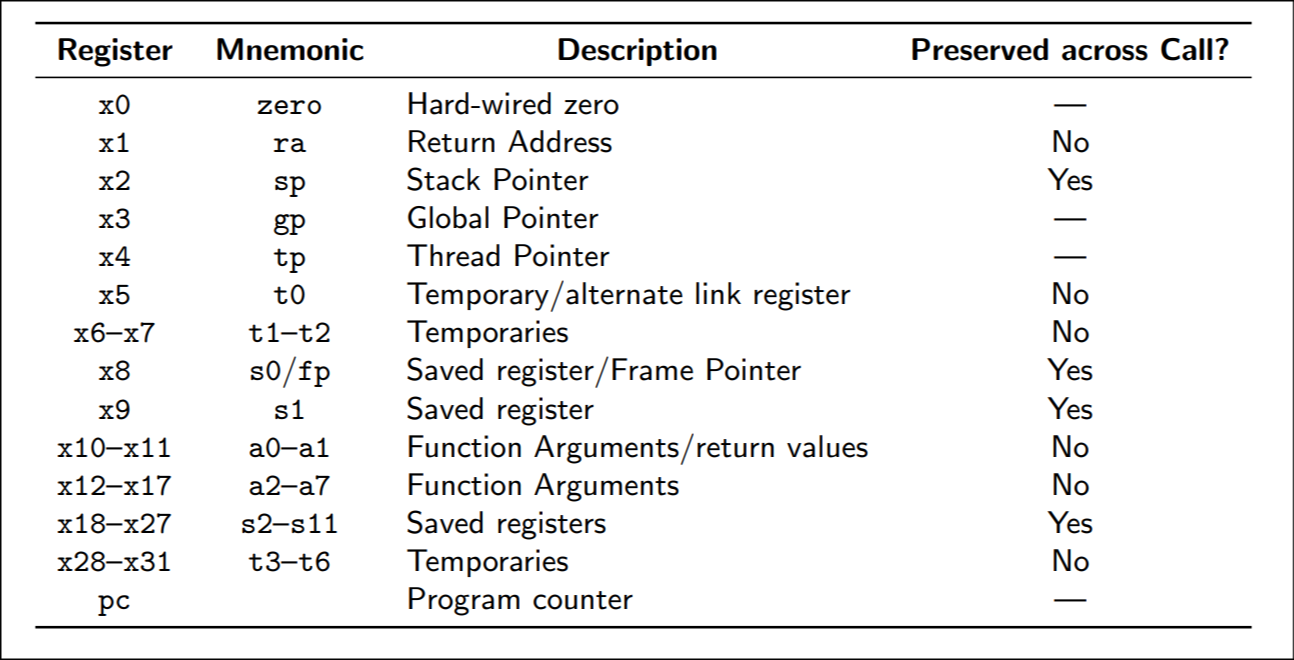
\includegraphics[scale=0.3]{screenshots/2025-10-11_7.png}
\end{center}

















